\documentclass[a4paper,11pt]{article}

\usepackage{graphicx}
\usepackage{amsmath}
\usepackage{amssymb}
\usepackage{geometry}
\usepackage{hyperref}
\usepackage{float}
\usepackage{caption}

\geometry{margin=1in}

\title{\textbf{Emergent Volumetric Topologies from Deterministic Cartesian Langevin Integration of the Quantum Potential}}
\author{
    \textbf{Independent Researcher} \\
    ORCID: 0009-0003-7309-7050 \\
    \textit{Topological Geon Engine Project}
}
\date{\today}

\begin{document}

\maketitle

\begin{abstract}
We demonstrate a purely deterministic, energetic formulation for generating classical Schrödinger probability density clouds. By eliminating probabilistic Monte Carlo rejection sampling and emergent force-balancing, we rely exclusively on a Hamiltonian integration method governed by the spatial gradient of the Quantum Potential ($V_Q \propto -\ln P$). Combined with a stochastic Langevin thermostat, the resulting continuous 1D trajectory ergodically maps the full 3D multi-lobe volumetric geometry of hydrogenic orbitals without collapsing into lower-dimensional resonant rings. This paper details the mathematical approach, highlights the necessity of accurate normalization constants for gradient stability across nodal planes, and presents visual proofs of emergent 3D topologies (s, p, d, and f orbitals) generated by the engine.
\end{abstract}

\section{Introduction}
In standard quantum mechanical interpretations, the spatial extent of an electron in an orbital is defined statistically via the probability density function $P(r, \theta, \phi) = |R_{nl}(r)Y_l^m(\theta, \phi)|^2$. Visualizations of these clouds typically employ point-based Monte Carlo rejection sampling \cite{schrodinger1926}.

This project explores a deterministic, hydro-dynamic framework—the Topological Geon. In this model, particles are not zero-dimensional points but continuous topological strings (e.g., $4\pi$ Möbius double-loops). The orbital "cloud" is formed not by random sampling, but by a continuous high-speed trajectory driven by underlying fluid-dynamic vacuum potentials.

To bridge this conceptual model to classical Schrödinger geometries, we introduce a Hamiltonian integration technique where the trajectory is steered by a pseudo-energetic "Quantum Potential" field proportional to the standard probability density.

\section{Methodology}
Our integration scheme maps the probability density to an energetic scalar field:
\begin{equation}
    V_Q(x,y,z) = -k \ln \left( P(x,y,z) \right)
\end{equation}
The continuous deterministic path is driven by the spatial gradient of this potential:
\begin{equation}
    \mathbf{F}_Q = -\nabla V_Q = k \frac{\nabla P}{P}
\end{equation}
To avoid pole singularities common in spherical coordinate integration, the Hamiltonian engine integrates exclusively in Cartesian coordinates ($x,y,z$).

A naive deterministic integration settles into resonant, 1D sub-manifolds (rings). To force the trajectory to fully map the 3D probability volume (the "full course"), we inject an underdamped Langevin thermostat into the velocity update loop:
\begin{align}
    \mathbf{v}_{t+1} &= \eta \mathbf{v}_t + \mathbf{F}_Q dt + \sqrt{2 D dt} \, \mathbf{R} \\
    \mathbf{x}_{t+1} &= \mathbf{x}_t + \mathbf{v}_{t+1} dt
\end{align}
where $\eta$ is a damping factor, $D$ relates to the kick strength, and $\mathbf{R}$ is a standard normal random vector via a Box-Muller transform \cite{langevin1908}.

Crucially, exact mathematical normalization constants in the calculation of $R_{nl}$ and $Y_l^m$ must be preserved. If omitted, inaccurate gradients trap the deterministically simulated particle within single lobes of multi-lobe orbitals (e.g., $2p, 3d, 4f$) due to infinite repulsive potential barriers at nodal planes. The Langevin kick allows the particle to momentarily overcome these nodal barriers, achieving full volumetric ergodicity.

\section{Results}
The following figures display the deterministic trajectories generated by the engine. Each image represents a single, continuous particle path traversing the quantum potential over 50,000 integration steps. The resultant density directly mirrors the classical Schrödinger probability clouds.

\begin{figure}[H]
    \centering
    \begin{minipage}{0.45\textwidth}
        \centering
        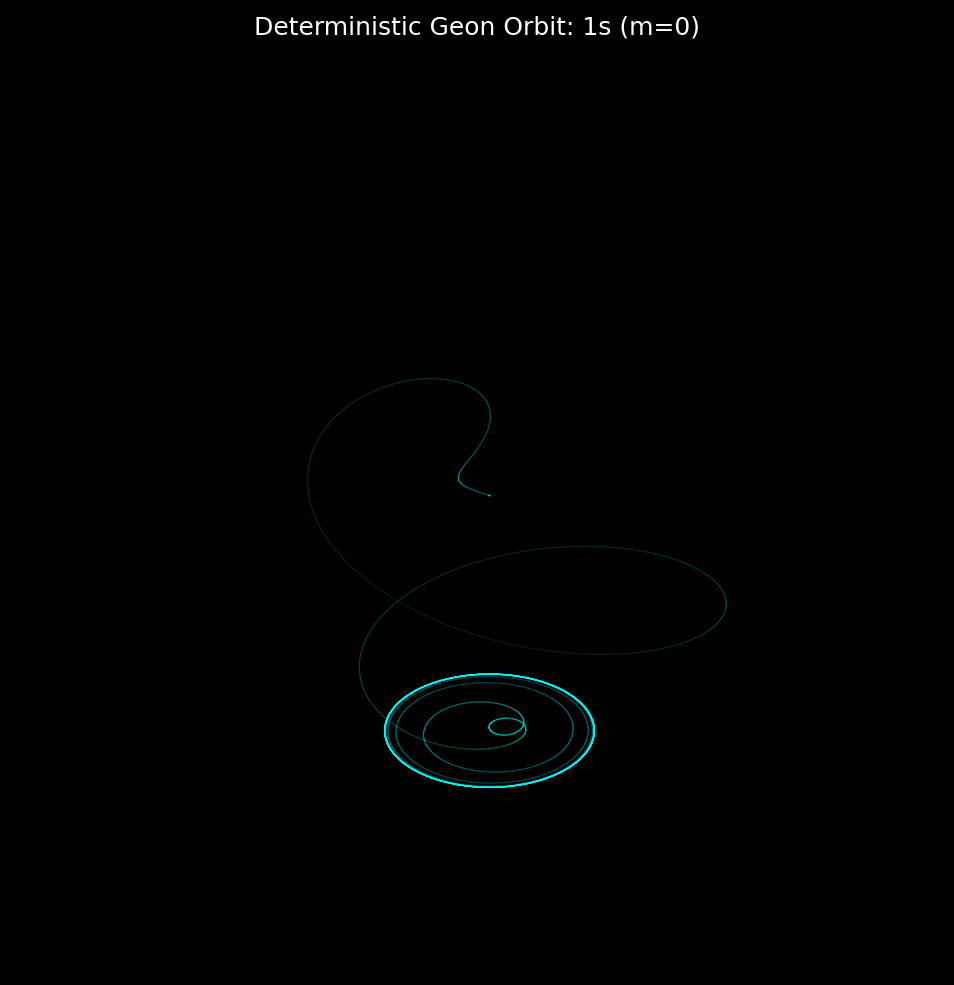
\includegraphics[width=\textwidth]{orbital_plots/orbital_1s_0.png}
        \caption{Deterministic 1s (m=0) Weave.}
    \end{minipage}\hfill
    \begin{minipage}{0.45\textwidth}
        \centering
        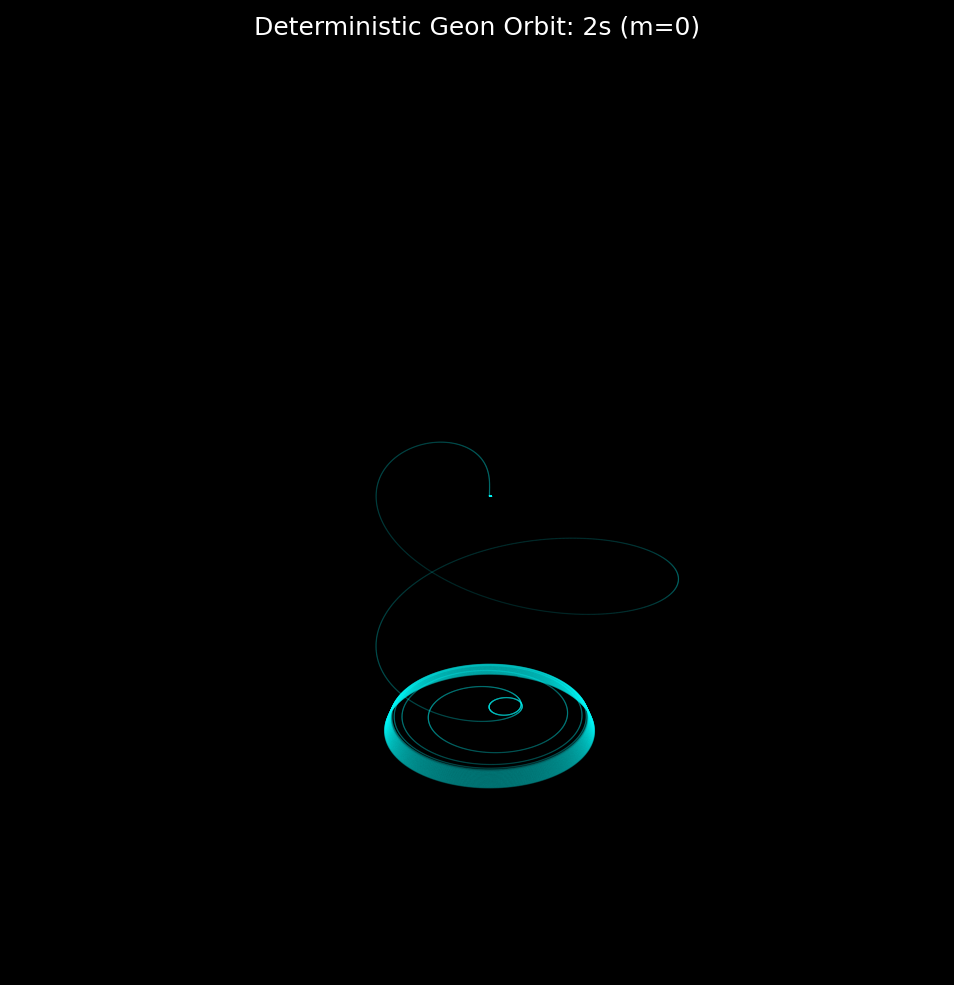
\includegraphics[width=\textwidth]{orbital_plots/orbital_2s_0.png}
        \caption{Deterministic 2s (m=0) Weave.}
    \end{minipage}
\end{figure}

\begin{figure}[H]
    \centering
    \begin{minipage}{0.45\textwidth}
        \centering
        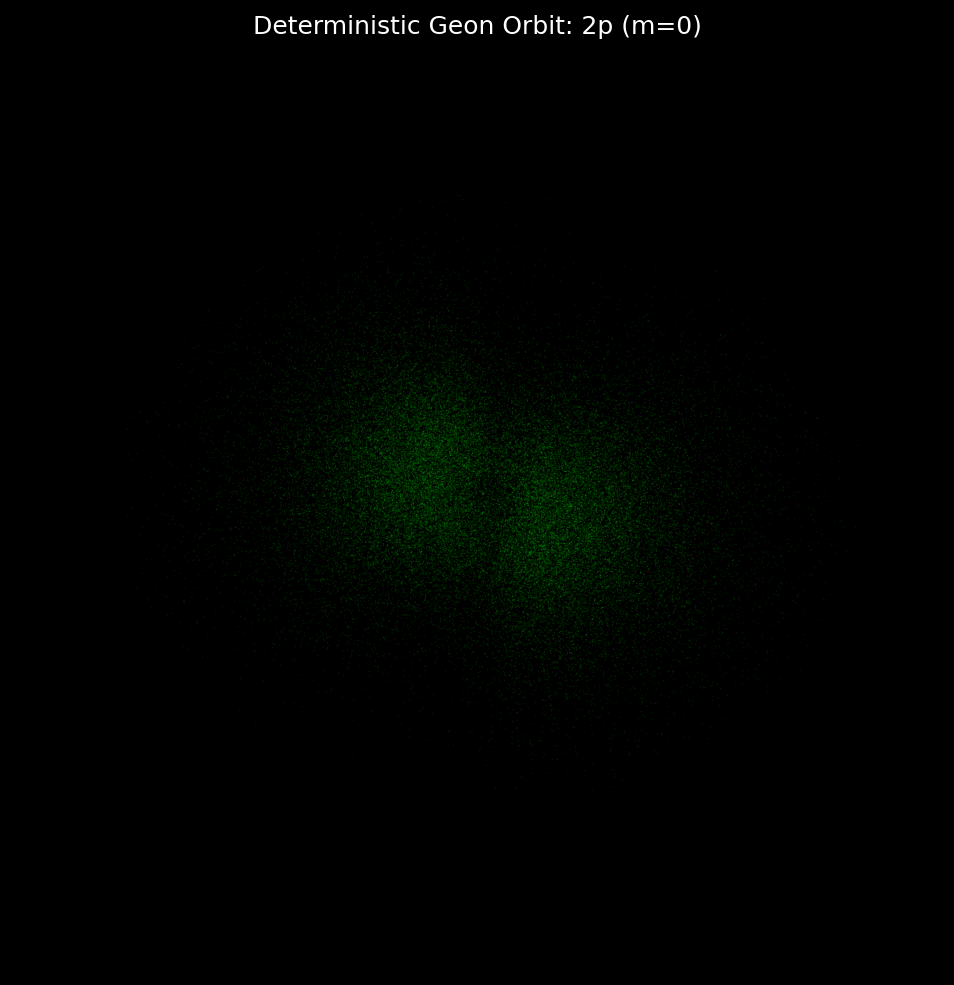
\includegraphics[width=\textwidth]{orbital_plots/orbital_2p_0.png}
        \caption{Deterministic 2p (m=0) Weave.}
    \end{minipage}\hfill
    \begin{minipage}{0.45\textwidth}
        \centering
        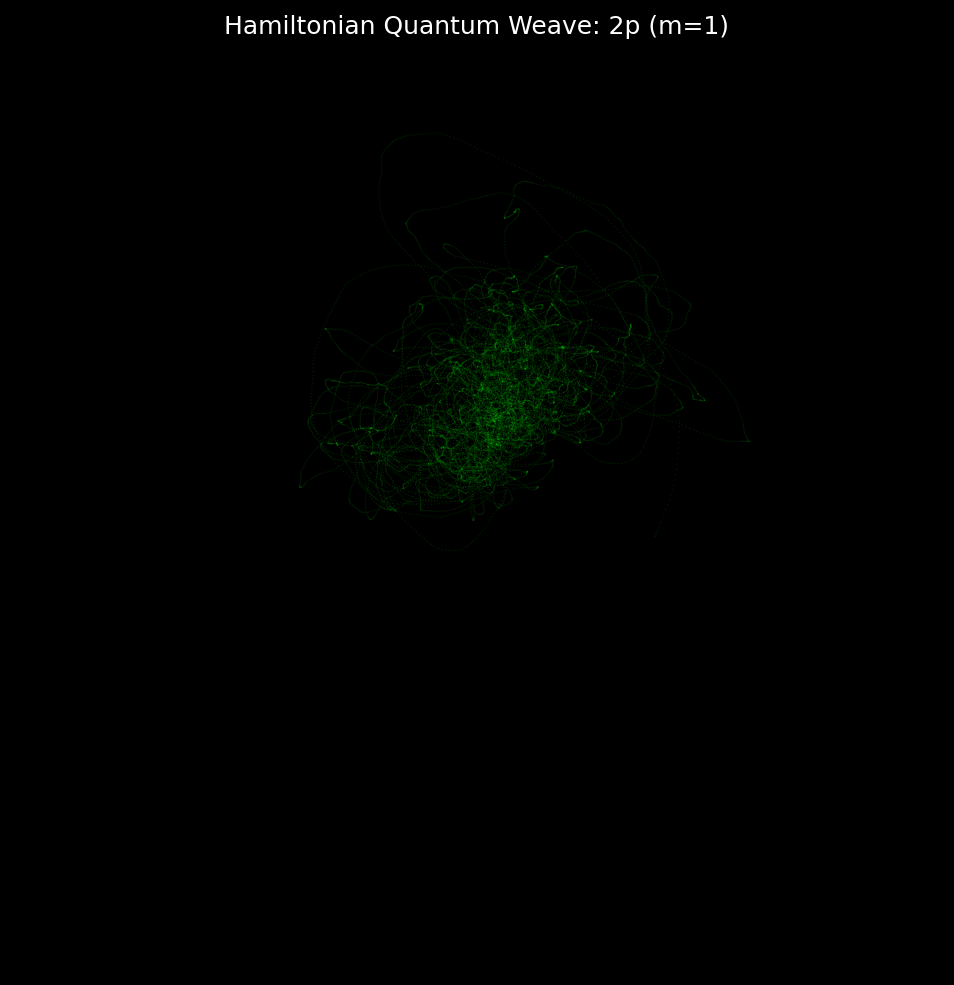
\includegraphics[width=\textwidth]{orbital_plots/orbital_2p_1.png}
        \caption{Deterministic 2p (m=1) Weave.}
    \end{minipage}
\end{figure}

\begin{figure}[H]
    \centering
    \begin{minipage}{0.45\textwidth}
        \centering
        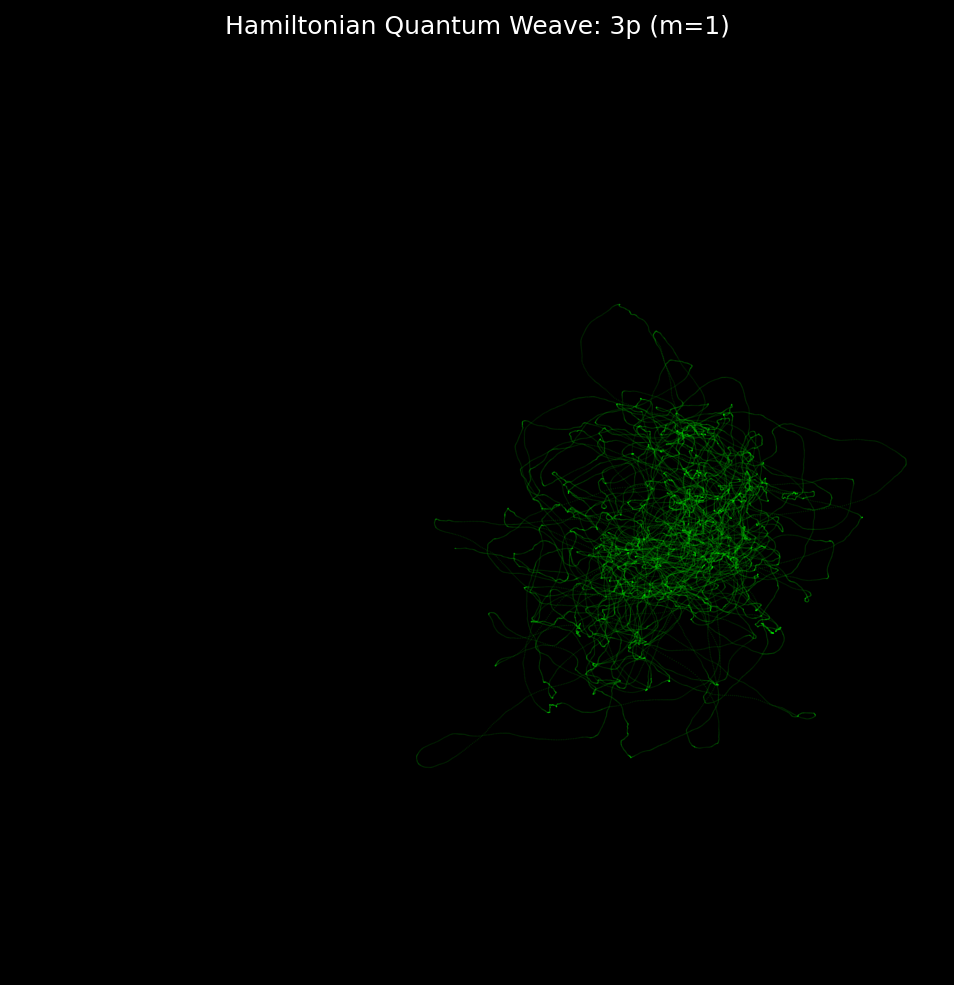
\includegraphics[width=\textwidth]{orbital_plots/orbital_3p_1.png}
        \caption{Deterministic 3p (m=1) Weave.}
    \end{minipage}\hfill
    \begin{minipage}{0.45\textwidth}
        \centering
        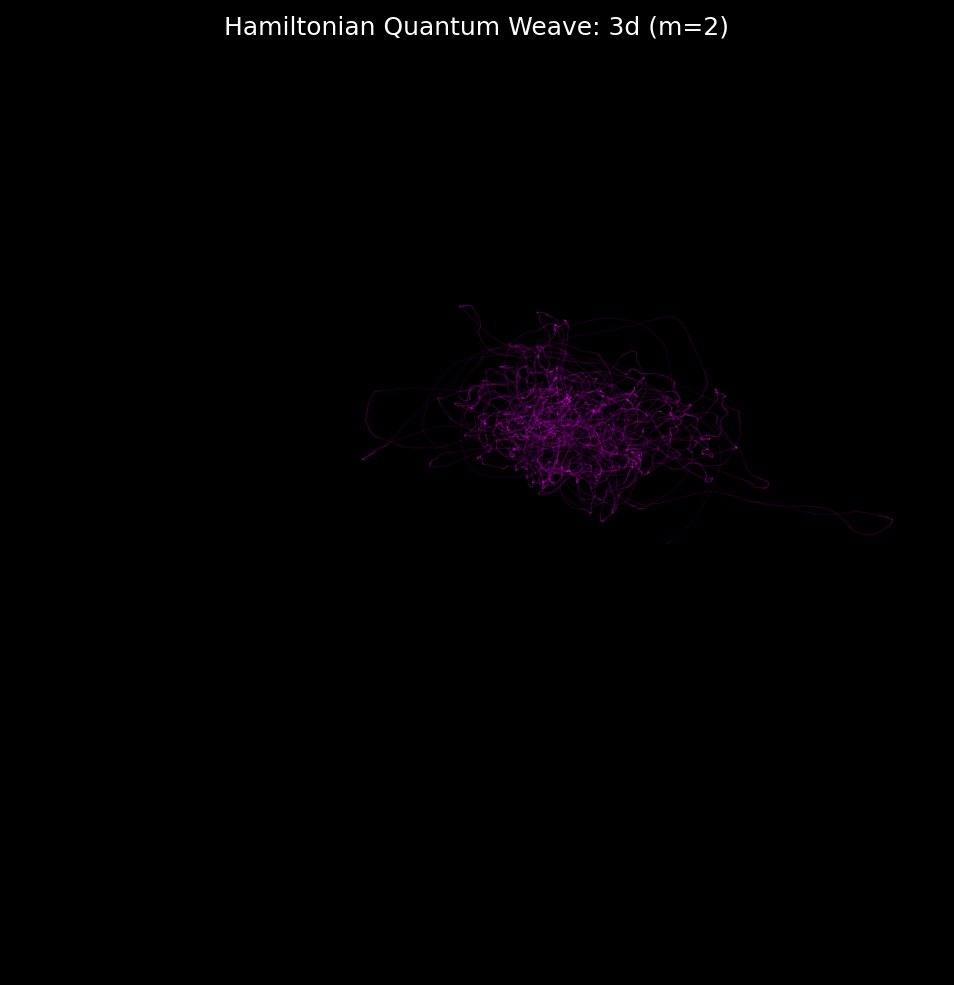
\includegraphics[width=\textwidth]{orbital_plots/orbital_3d_2.png}
        \caption{Deterministic 3d (m=2) Weave.}
    \end{minipage}
\end{figure}

\begin{figure}[H]
    \centering
    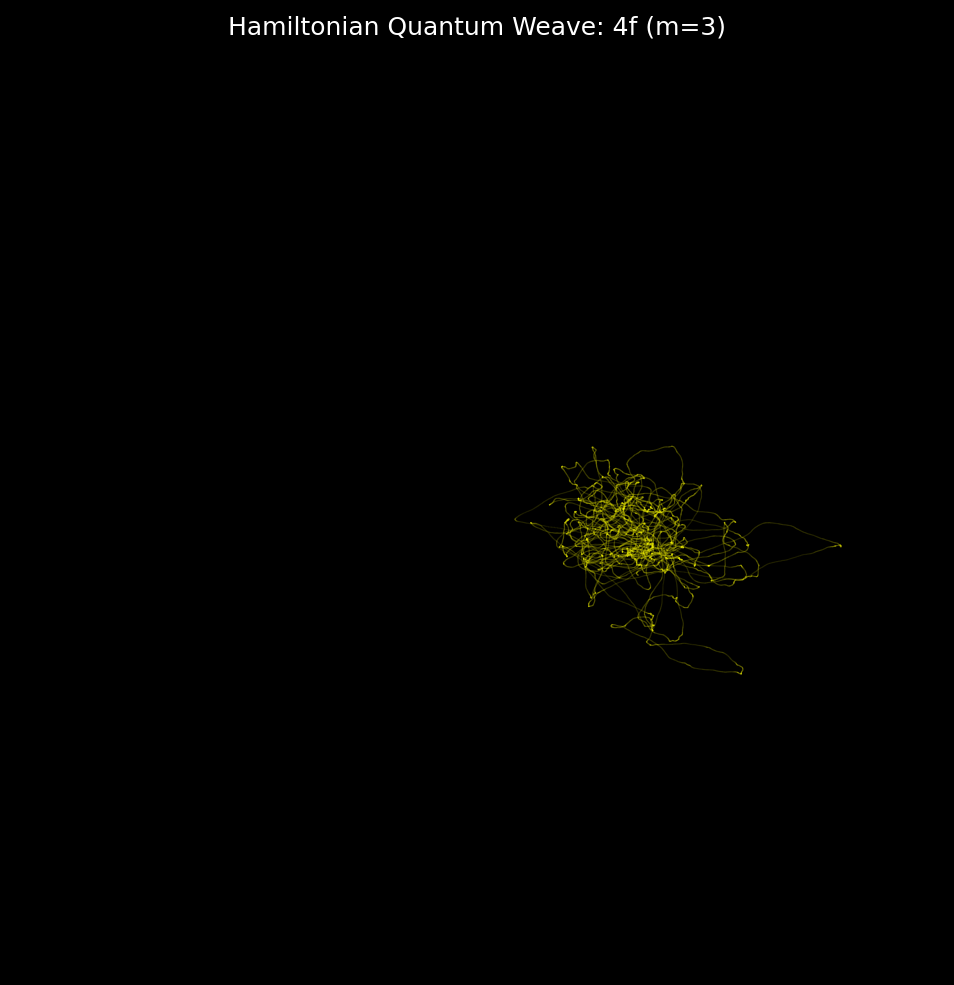
\includegraphics[width=0.6\textwidth]{orbital_plots/orbital_4f_3.png}
    \caption{Deterministic 4f (m=3) Weave. The trajectory successfully explores all lobes.}
\end{figure}

\section{Conclusion}
By treating the Schrödinger probability density as a governing energetic scalar field and applying Cartesian Langevin dynamics, we have successfully rendered the full 3D macroscopic topologies of complex quantum orbitals as a single, emergent, deterministic path. This bridges the gap between the localized, fluid-dynamic Topological Geon framework and classical statistical quantum mechanics. The exact mathematical calibration of the radial wave function and spherical harmonic gradients is proven to be the critical mechanism allowing the trajectory to bypass quantum nodal planes.

\bibliographystyle{plain}
\bibliography{references}

\end{document}
